% ------------------------------------------------------------
% UFOP – Prova (estilo conciso, sem seções, sem instruções)
% ------------------------------------------------------------
\documentclass[12pt,a4paper]{article}
\usepackage[T1]{fontenc}
\usepackage[utf8]{inputenc}
\usepackage[brazil]{babel}
\usepackage{geometry}
\geometry{margin=2.5cm}
\usepackage{amsmath,amssymb,booktabs}
\usepackage{enumitem}
\usepackage{fancyhdr}
\usepackage{graphicx}
\usepackage{subcaption} % For subfigures

\pagestyle{fancy}
\fancyhf{}
\lhead{Universidade Federal de Ouro Preto}
\rhead{\thepage}

\begin{document}

\begin{center}
  {\Large \textbf{BCC 740 -- Inteligência Artificial}}\\[2pt]
  {\large \textbf{Prova 4}}\\[4pt]
\end{center}


*Verifique se a sua folha de questões possui 14 questões.

\begin{enumerate}[leftmargin=0.55cm,itemsep=0.65em]

  \item Utilizando a árvore de decisão apresentada na Figura \ref{fig:dt}, classifique os exemplos descritos na Tabela \ref{tab:e19e20}.


  \begin{figure}[!ht]
    \centering
    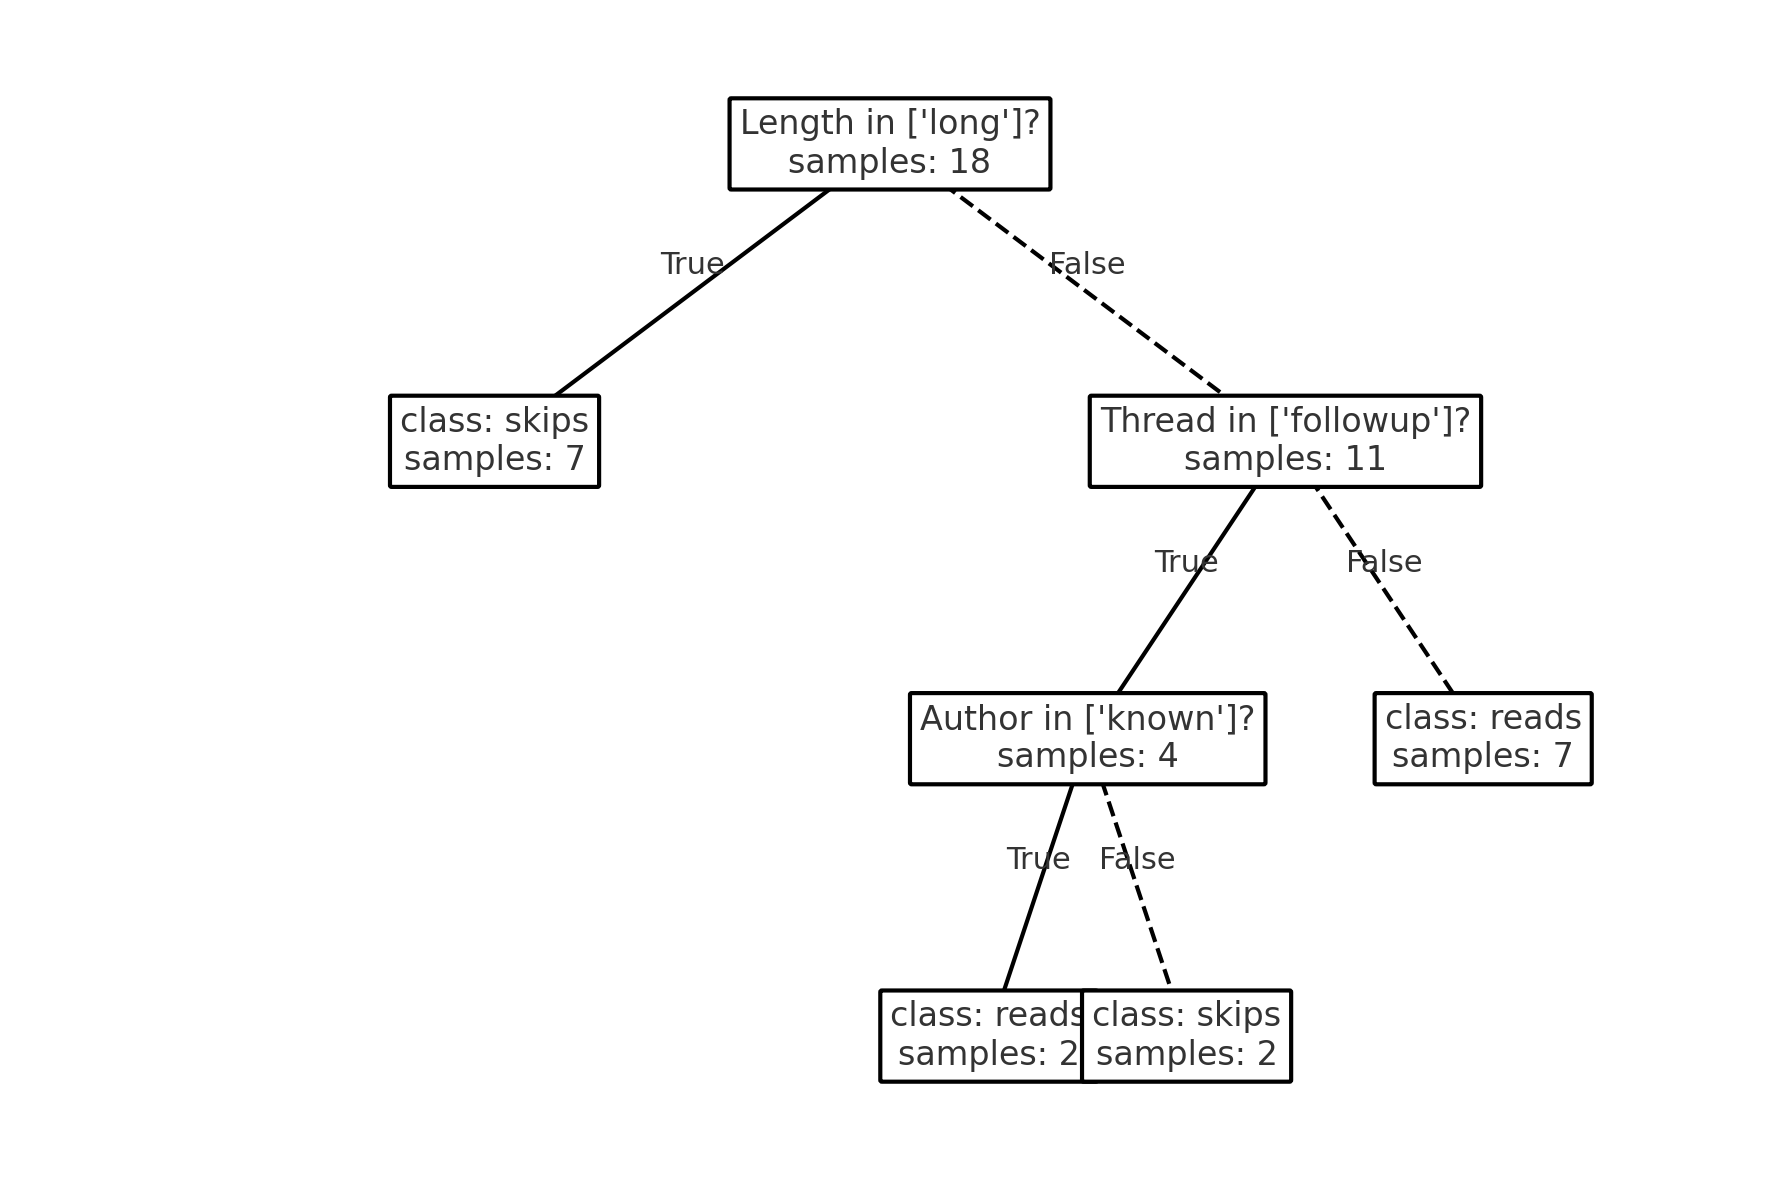
\includegraphics[width=0.95\textwidth]{dt.png}
    \caption{Árvore de decisão}
    \label{fig:dt}
  \end{figure}


  \begin{table}[h!]
    \centering
    \begin{tabular}{lcccc}
    \hline
    \textbf{Example} & \textbf{Author} & \textbf{Thread} & \textbf{Length} & \textbf{Where\_read} \\
    \hline
    e19 & unknown & new      & long  & work \\
    e20 & unknown & followup & short & home \\
    \hline
    \end{tabular}
    \caption{Attribute values for e19 and e20.}
    \label{tab:e19e20}
  \end{table}

  \item Considere o treinamento de uma rede neural via descida do gradiente. Dados o vetor de pesos e \textit{biases} $\mathbf{w} = [0.9,0.65,1.67,9.15,7,34,9.11]^T$, a taxa de aprendizado $\eta = 0.1$ e o gradiente da \textit{loss} $\nabla L = [0.1,0.2,0.33,0.4,0.12,0.15,1]$, qual será o novo vetor de pesos?
  
  \item O que acontece com o processo de otimização se a taxa de aprendizado (\textit{learning rate}) for muito alta? E se for muito baixa?

  \item Quais critérios podem ser utilizados para escolher a função de ativação de um neurônio em uma rede neural artificial?
  
  \item Defina uma estratégia de regularização que funcione exclusivamente para redes neurais artificiais e outra que funcione exclusivamente para árvores de decisão.
  
  \item Defina uma estratégia de regularização que seja aplicável tanto a redes neurais artificiais quanto a árvores de decisão.
  
  \item Indique uma estratégia de regularização que atua na função de perda. Explique como ela regulariza o modelo. 
  
  \item Observe as curvas de aprendizado de dois algoritmos de aprendizagem de máquina. Quais são os nomes dos processos ilustrados em cada figura?
  
  \begin{figure}[htbp]
      \centering
      % --- Underfitting ---
      \begin{subfigure}[b]{0.48\textwidth}
          \centering
          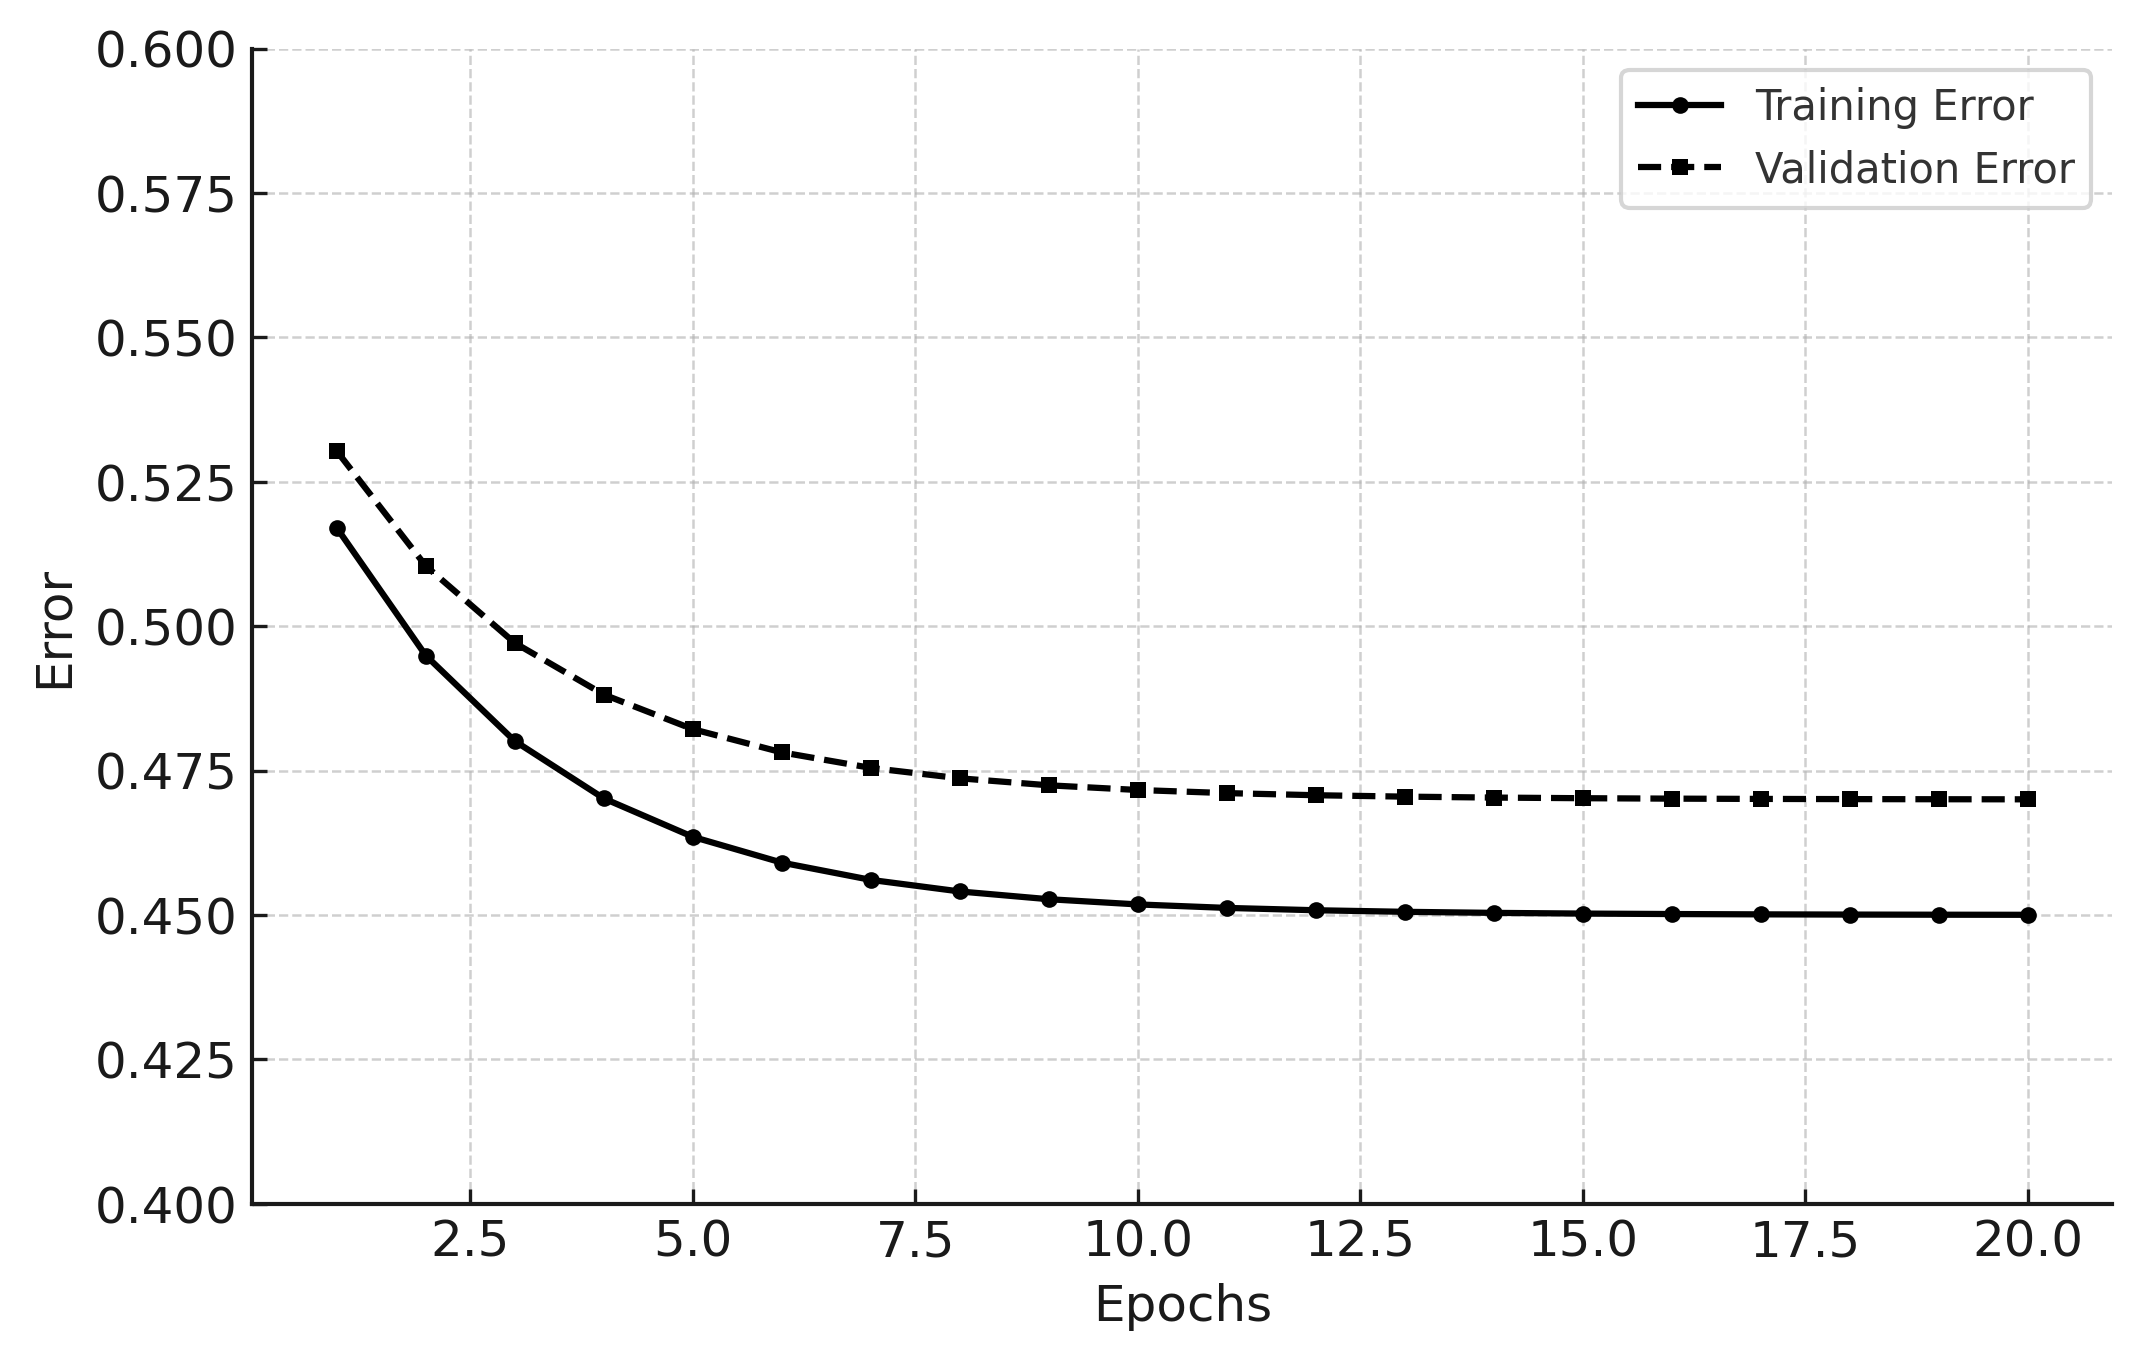
\includegraphics[width=\textwidth]{under.png}
          \caption{Algoritmo A}
          \label{fig:underfitting}
      \end{subfigure}
      \hfill
      % --- Overfitting ---
      \begin{subfigure}[b]{0.48\textwidth}
          \centering
          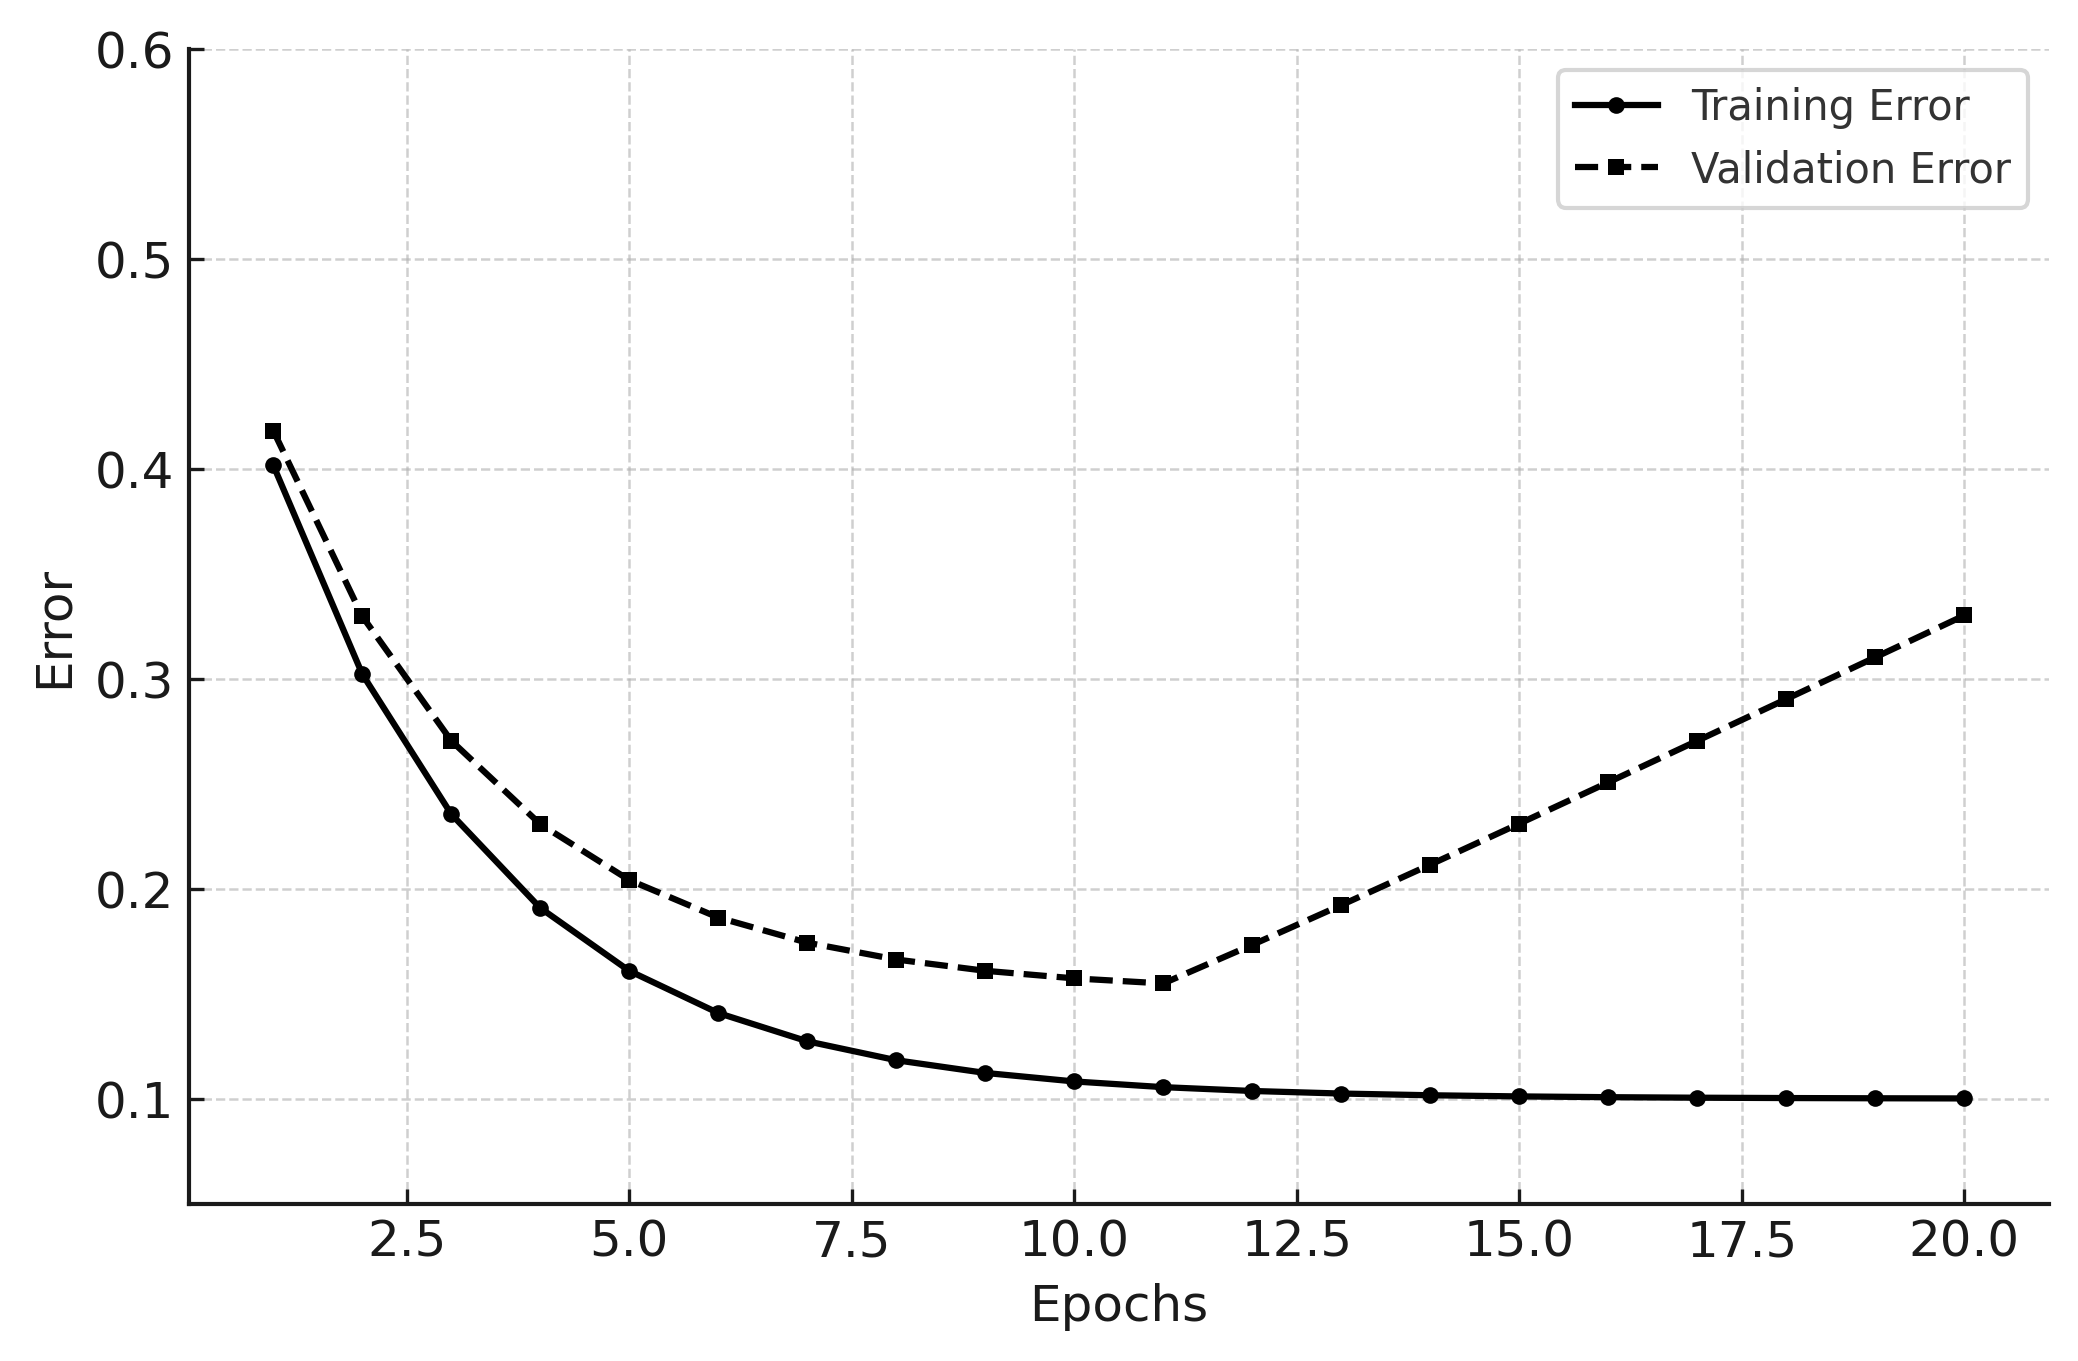
\includegraphics[width=\textwidth]{over.png}
          \caption{Algoritmo B}
          \label{fig:overfitting}
      \end{subfigure}
      
      \caption{Curvas de aprendizado típicas}
      \label{fig:learning_curves}
  \end{figure}

  \item Ao treinar um modelo de aprendizagem de máquina, você verificou que o algoritmo de treinamento apresenta dificuldade em minimizar o erro (\textit{loss}). O que pode ser feito para mitigar esse problema?

  \item Quais funções de perda (\textit{loss}) podem ser utilizadas para treinar uma rede neural em um problema de regressão? E em problemas de classificação?
  
  \item Quais são as limitações de avaliar um modelo de aprendizagem de máquina usando apenas um único \textit{holdout}? Indique um método mais adequado de avaliação e explique como ele resolve as limitações do \textit{holdout}.
  
  \item O que é \textit{data leakage}? Dê dois exemplos comuns e explique como evitá-los.
  
  \item Em um problema desbalanceado, por que a acurácia pode mascarar o \textit{overfitting}? Sugira métricas alternativas.
  
  \item Descreva a função dos conjuntos de treinamento, validação e teste.

\end{enumerate}

\end{document}
